\chapter{基于多维度特征的PE识别结果与分析}
\section{引言}
此前的论文内容已经分别从机器学习的输入特征及机器学习的模型算法等方面进行铺垫介绍。本章将具体介绍利用前文提出的脉搏波的特征集合、使用多种机器学习算法
构建并评估子痫前期的一般识别模型。此外, 本章也对评估机器学习模型性能表现的一般指标进行了介绍。
\section{监督学习模型评估指标}
一、混淆矩阵

混淆矩阵(confusion matrix)是评估分类器分类效果优劣的常用工具\cite{Zhou2016,Aurélien2018}。其总体思路就是分别统计A类别实例被划分成B类别实例的数目。理论上混淆矩阵的行列没有上限,而在实际应用中,二分类任务的混淆矩阵是最常见的。
此时,将样例依据其真实所属类别与分类器预测类别进行组合可得到四种结果:真阳性(true positive,TP)、假阳性(false positive,FP)、真阴性(true negative,TN)及假阴性(false negative,TN),如\autoref{tab:cm}所示。此时显然有
$TP+FP+TN+FN=\text{样例总数}$。
\begin{table}[htbp]
      \centering
      \caption{\label{tab:cm}二分类任务的混淆矩阵}
      \begin{tabular}{ccc}
      \toprule
      \multicolumn{1}{c}{\multirow{2}[4]{*}{\textbf{真实情况}}} & \multicolumn{2}{c}{\textbf{预测结果}} \\
            \cmidrule{2-3}          & 阳性(1) & 阴性(0) \\
      \midrule
      阳性(1) & 真阳性(TP) & 假阴性(FN) \\
      阴性(0) & 假阳性(FP) & 真阴性(TN) \\
      \bottomrule
      \end{tabular}%
\end{table}%

为量化分类器的具体性能,人们在混淆矩阵的基础上衍生定义了一系列数字指标,包括查全率(recall)、查准率(precison)、准确率(accuracy)及特异性(specificity)等,如\autoref{equ:measures}所示。
\begin{equation}
      \label{equ:measures}
      \left \{
      \begin{aligned}
            Recall      &=\frac{TP}{TP+FN}         \\
            Precison    &=\frac{TP}{TP+FP}          \\
            Accuracy    &=\frac{TP+TN}{TP+FP+TN+FN} \\
            Specificity &=\frac{TN}{TN+FP}       \\
      \end{aligned}
      \right.
\end{equation}
其中,查全率亦称召回率、灵敏性(sensitivity)或真阳性率(true positive rate,TPR),查准率亦称精准率,特异性亦称真阴性率。查全率与查准率是应用的最广泛的两个指标\cite{Zhou2016,Aurélien2018}。
一般而言,查全率与查准率是对相互矛盾的度量指标,一个指标性能的提高意味着另一个指标性能的下降。通常只有在简单分类任务中,
才能同时获得较高的查准率与查全率。这称为精度-召回率权衡。为评估查全率与查准率均不相等的分类器性能,人们进一步定义了$F_1\text{分数}$,如\autoref{equ:f1}所示。
\begin{equation}
      \label{equ:f1}
      F_1=\frac{2}{\frac{1}{Precison}+\frac{1}{Recall}}=\frac{2\cdot Precison\cdot Recall}{Precison+Recall}=\frac{TP}{TP+\frac{FN+FP}{2}}
\end{equation}
$F_1\text{分数}$是召回率与精准率的谐波均值。召回率与精准率相近的分类器易获得更高的$F_1\text{分数}$。

在评估分类器性能时需要根据场景,从\autoref{equ:measures}与\autoref{equ:f1}中灵活选取恰当的评价指标。

二、ROC曲线、AUC与约登指数

受试者工作特征(Receiver Operating Characteristic,ROC)曲线是另一种常用于二分类问题的分析工具。ROC绘制的是真阳性率和假阳性率(false positive rate,FPR)之间的变化关系,其中
\begin{equation}
      \label{equ:fpr}
      FPR=\frac{TN}{TN+FP}=1-Specificity
\end{equation}
因此,ROC曲线也被称为灵敏度与1-特异性曲线。绘制曲线时,以分类器的预测结果对样例进行升序排列,依次将样本作为阳性进行预测,计算对应的TPR与FPR后,可得一坐标点$({FPR}_i,{TPR}_i)$,最后将所有坐标点连线即可,如\autoref{fig:roc}所示。
其中,虚线表示纯随机分类器的ROC曲线,理想性能的分类器应无限逼近左上角,即坐标点$(0,1)$。
\begin{figure}[htbp]
      \centering
      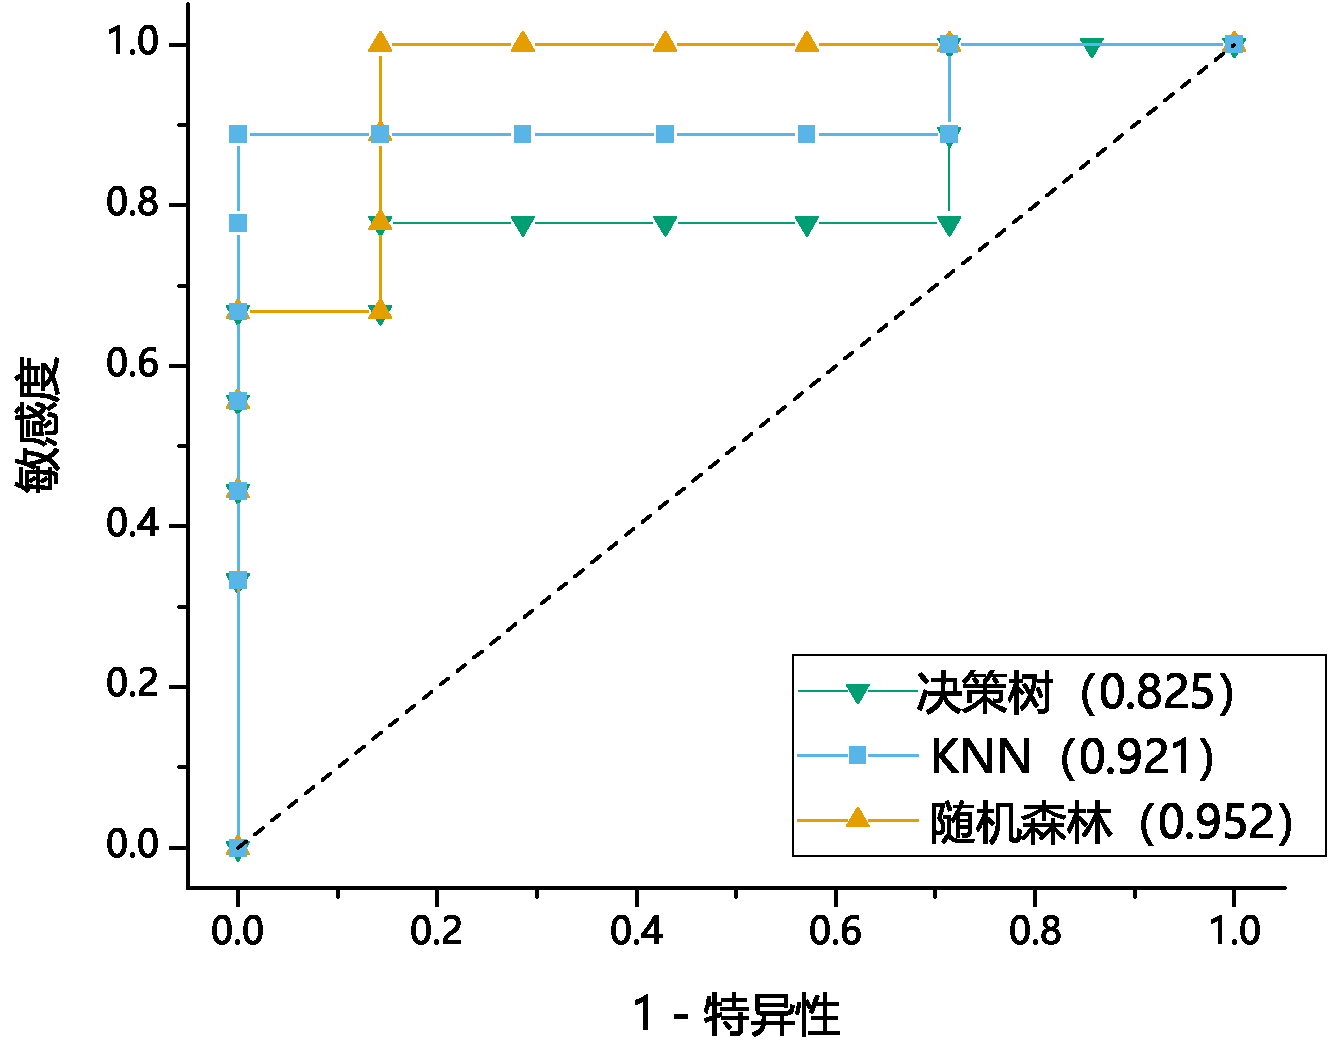
\includegraphics[width=.6\linewidth]{data_plan/roc}
      \caption[ROC曲线与AUC数值]{\label{fig:roc}ROC曲线与AUC数值。各分类器的AUC具体数值参见图例。}
\end{figure}

在衡量多个分类器性能优劣时,常将分类器对应的ROC曲线下面积作为判据,即为AUC(Area Under Curve)。纯随机分类器ROC的AUC数值为0.5,而理想分类器ROC的AUC数值为1,如\autoref{fig:roc}所示。

此外,约登指数(Youden Index)也是用来评价分类器效果的一个指标。若在评估分类器性能时,给予将分类器假阴性和假阳性以相同权重,即可应用约登指数
\begin{equation}
      \label{equ:yi}
      \begin{aligned}
            YI&=Sensitivity-(1-Specificity)\\
            &=Sensitivity+Specificity-1
      \end{aligned}
\end{equation}
一般认为,当YI取值最大时,此时对应的分类阈值为最佳阈值\cite{cwl}。
\section{监督学习算法的具体表现及分析}
\subsection{基于脉搏波时域特征集\Rnum{1}的结果及分析}
一、按照全部波形抽样

1. 模型初筛

为检验借助脉搏波时域特征集\Rnum{1}中的各项时域参数能否识别出孕妇是否患有子痫前期,本研究首先基于全部波形分层抽样的数据样本进行了监督学习算法的试探性研究\cite{scikit-learn}。
本研究共使用了随机梯度下降、决策树、K近邻、高斯朴素贝叶斯算法、逻辑回归、线性支持向量机、核支持向量机、C-支持向量机及多层感知机等9种基本分类算法进行模型探究。这些模型在进行初筛时,模型超参数均使用了默认设置\cite{scikit-learn}。
9种模型的初筛结果如\autoref{tab:model_screen}所示,其中训练集相关数据是对原始训练集数据经过5层交叉验证后得到的。

\begin{landscape}
      \zihao{-5}
      \begin{longtable}{m{3cm}<{\centering}m{1.7cm}<{\centering}m{2.3cm}<{\centering}m{1cm}<{\centering}m{1cm}<{\centering}m{1cm}<{\centering}m{1cm}<{\centering}m{1cm}<{\centering}m{2cm}<{\centering}m{1cm}<{\centering}m{1cm}<{\centering}m{1cm}<{\centering}m{1cm}<{\centering}}
            \caption{初筛结果}\\
            \label{tab:model_screen}\\
            \toprule
            &  & \multicolumn{6}{c}{\textbf{训练集(5层交叉验证)}} & \multicolumn{5}{c}{\textbf{验证集}}                                                                                                                                                                                                      \\
            \multirow{-2}{*}{\textbf{模型类型}} & \multirow{-2}{*}{\textbf{训练时间}} & \textbf{混淆矩阵} &  \textbf{精确率} &  \textbf{召回率} &  \textbf{F1值} &  \textbf{准确率} &  \textbf{AUC} &  \textbf{混淆矩阵} &  \textbf{精确率} &  \textbf{召回率} &  \textbf{F1值} &  \textbf{准确率}    \\
            \midrule
            \endfirsthead
            \caption[]{(续)}\\
            \midrule
            &  & \multicolumn{6}{c}{\textbf{训练集(5层交叉验证)}} & \multicolumn{5}{c}{\textbf{验证集}}                                                                                                                                                                                                      \\
            \multirow{-2}{*}{\textbf{模型类型}} & \multirow{-2}{*}{\textbf{训练时间}} & \textbf{混淆矩阵} &  \textbf{精确率} &  \textbf{召回率} &  \textbf{F1值} &  \textbf{准确率} &  \textbf{AUC} &  \textbf{混淆矩阵} &  \textbf{精确率} &  \textbf{召回率} &  \textbf{F1值} &  \textbf{准确率}    \\
            \midrule
            \endhead 
            \midrule
            \endfoot
            \bottomrule
            \endlastfoot
            随机梯度下降      &   6.17 s  &     $\left[ \begin{array}{cc} 2165 & 380 \\ 1164 & 2582 \end{array} \right]$ & 87.2\% & 68.9\% & 77.0\% & 75.5\% & 0.876 &
            $\left[ \begin{array}{cc} 328 & 308 \\ 22 & 915 \end{array} \right]$ & 74.8\% & 97.7\% & 84.7\% & 79.0\% \\
            决策树            &   5.24 s  &     $\left[ \begin{array}{cc} 2241 & 304 \\ 635 & 3111 \end{array} \right]$ & 91.1\% & 83.0\% & 86.9\% & 85.1\% & 0.907 &
            $\left[ \begin{array}{cc} 584 & 52 \\ 174 & 763 \end{array} \right]$ & 93.6\% & 81.4\% & 87.1\% & 85.6\% \\
            K近邻算法      &   3.08 s  &     $\left[ \begin{array}{cc} 2347 & 198 \\ 237 & 3509 \end{array} \right]$ & 94.7\% & 93.7\% & 94.2\% & 93.1\% & 0.974 &
            $\left[ \begin{array}{cc} 594 & 42 \\ 63 & 874 \end{array} \right]$ & 95.4\% & 93.3\% & 94.3\% & 93.3\% \\
            高斯朴素贝叶斯算法      &   1.22 s  &     $\left[ \begin{array}{cc} 2215 & 320 \\ 1354 & 2392 \end{array} \right]$ & 87.9\% & 63.9\% & 74.0\% & 73.2\% & 0.838 &
            $\left[ \begin{array}{cc} 569 & 67 \\ 328 & 609 \end{array} \right]$ & 90.1\% & 65.0\% & 75.5\% & 74.9\% \\
            逻辑回归算法      &   203.0 s  &     $\left[ \begin{array}{cc} 2174 & 371 \\ 347 & 3399 \end{array} \right]$ & 90.2\% & 90.7\% & 90.4\% & 88.6\% & 0.950 &
            $\left[ \begin{array}{cc} 573 & 63 \\ 66 & 871 \end{array} \right]$ & 93.3\% & 93.0\% & 93.1\% & 91.8\% \\
            线性支持向量机      &   47.22 s  &     $\left[ \begin{array}{cc} 1658 & 887 \\ 254 & 3492 \end{array} \right]$ & 79.7\% & 93.2\% & 86.0\% & 81.9\% & 0.917 &
            $\left[ \begin{array}{cc} 603 & 33 \\ 170 & 767 \end{array} \right]$ & 95.9\% & 81.9\% & 88.3\% & 87.1\% \\
            核支持向量机      &   60.28 s  &     $\left[ \begin{array}{cc} 1828 & 717 \\ 363 & 3383 \end{array} \right]$ & 82.5\% & 90.3\% & 86.2\% & 82.8\% & 0.916 &
            $\left[ \begin{array}{cc} 484 & 152 \\ 81 & 856 \end{array} \right]$ & 84.9\% & 91.4\% & 88.0\% & 85.2\% \\
            C-支持向量机      &   42.47 s  &     $\left[ \begin{array}{cc} 1914 & 631 \\ 354 & 3392 \end{array} \right]$ & 84.3\% & 90.5\% & 87.3\% & 84.3\% & 0.929 &
            $\left[ \begin{array}{cc} 510 & 126 \\ 86 & 851 \end{array} \right]$ & 87.1\% & 90.8\% & 88.9\% & 86.5\% \\
            多层感知机      &   26.8 s  &     $\left[ \begin{array}{cc} 1982 & 563 \\ 906 & 2840 \end{array} \right]$ & 83.5\% & 75.8\% & 79.5\% & 76.6\% & 0.905 &
            $\left[ \begin{array}{cc} 534 & 102 \\ 83 & 854 \end{array} \right]$ & 89.3\% & 91.1\% & 90.2\% & 88.2\% \\
      \end{longtable}
\end{landscape}

\begin{landscape}
      \zihao{-5}
      \begin{longtable}{m{3cm}<{\centering}m{5cm}<{\centering}m{1cm}<{\centering}m{2cm}<{\centering}m{1cm}<{\centering}m{3cm}<{\centering}m{1cm}<{\centering}m{2cm}<{\centering}m{1cm}<{\centering}}
            \caption{超参数优化前后模型性能对比}\\
            \label{tab:super_para}\\
            \toprule
            \multicolumn{1}{c}{\multirow{3}{*}{\textbf{模型类型}}} & \multicolumn{1}{c}{\multirow{3}{*}{\textbf{超参数组合值域}}}    & \multicolumn{3}{c}{\textbf{优化前}}   & \multicolumn{1}{c}{\multirow{3}{*}{\textbf{最优超参数}}}   & \multicolumn{3}{c}{\textbf{优化后}} \\
            \multicolumn{1}{c}{} & \multicolumn{1}{c}{}     & \textbf{训练集} & \multicolumn{2}{c}{\textbf{测试集}} & \multicolumn{1}{c}{}   & \textbf{训练集} & \multicolumn{2}{c}{\textbf{测试集}}     \\
            \multicolumn{1}{c}{} & \multicolumn{1}{c}{}     & \textbf{AUC} & \textbf{混淆矩阵}    & \textbf{准确率} & \multicolumn{1}{c}{}    & \textbf{AUC} & \multicolumn{1}{c}{\textbf{混淆矩阵}}     & \textbf{准确率} \\
            \midrule
            \endfirsthead
            \caption[]{(续)}\\
            \midrule
            \multicolumn{1}{c}{\multirow{3}{*}{\textbf{模型类型}}} & \multicolumn{1}{c}{\multirow{3}{*}{\textbf{超参数组合值域}}}    & \multicolumn{3}{c}{\textbf{优化前}}   & \multicolumn{1}{c}{\multirow{3}{*}{\textbf{最优超参数}}}   & \multicolumn{3}{c}{\textbf{优化后}} \\
            \multicolumn{1}{c}{} & \multicolumn{1}{c}{}     & \textbf{训练集} & \multicolumn{2}{c}{\textbf{测试集}} & \multicolumn{1}{c}{}   & \textbf{训练集} & \multicolumn{2}{c}{\textbf{测试集}}     \\
            \multicolumn{1}{c}{} & \multicolumn{1}{c}{}     & \textbf{AUC} & \textbf{混淆矩阵}    & \textbf{准确率} & \multicolumn{1}{c}{}    & \textbf{AUC} & \multicolumn{1}{c}{\textbf{混淆矩阵}}     & \textbf{准确率} \\
            \endhead 
            \midrule
            \endfoot
            \bottomrule
            \endlastfoot
            % \multirow{2}{*}{随机梯度下降}                            & \multirow{2}{*}{\begin{tabular}[c]{@{}l@{}}loss:{[}hinge, log\_loss,   \\ log, modified\_huber, \\ squared\_hinge, perceptron, \\ squared\_error,  huber,\\  epsilon\_insensitive, \\ squared\_epsilon\_insensitive{]},\\    penalty:{[}l2,l1,elasticnet{]},\\   alpha:{[}0.001,0.0001,0.00001{]}\end{tabular}} & \multirow{2}{*}{0.876} & \multirow{2}{*}{$\left[ \begin{array}{cc} 328 & 308 \\ 22 & 915 \end{array} \right]$ } & \multirow{2}{*}{79.0\%} & \multirow{2}{*}{\begin{tabular}[c]{@{}c@{}}alpha=0.001, \\ loss=squared\_hinge,   \\ penalty=elasticnet\end{tabular}} & \multirow{2}{*}{0.918} & \multirow{2}{*}{$\left[ \begin{array}{cc} 631 & 5 \\ 393 & 544 \end{array} \right]$} & \multirow{2}{*}{74.7\%} \\
            % &                      &      &       &    &    &    &      &     \\
            随机梯度下降    & \begin{tabular}[c]{@{}l@{}}loss:{[}\textbf{hinge}, log\_loss,   \\ log, modified\_huber, \\ squared\_hinge, perceptron, \\ squared\_error,  huber,\\  epsilon\_insensitive, \\ squared\_epsilon\_insensitive{]},\\    penalty:{[}\textbf{l2},l1,elasticnet{]},\\   alpha:{[}0.001,\textbf{0.0001},0.00001{]}\end{tabular} & 0.876        & $\left[ \begin{array}{cc} 328 & 308 \\ 22 & 915 \end{array} \right]$ & 79.0\%       & \begin{tabular}[c]{@{}l@{}}alpha=0.001, \\ loss=squared\_hinge,   \\ penalty=elasticnet\end{tabular} & 0.918        & $\left[ \begin{array}{cc} 631 & 5 \\ 393 & 544 \end{array} \right]$ & 74.7\%       \\
            高斯朴素贝叶斯算法   & var\_smoothing:{[}1e-5,1e-7,\textbf{1e-9},1e-11{]}       & 0.838        & $\left[ \begin{array}{cc} 569 & 67 \\ 328 & 609 \end{array} \right]$ & 74.9\%       & var\_smoothing=1e-7,                   & 0.842        & $\left[ \begin{array}{cc} 568 & 68 \\ 328 & 609 \end{array} \right]$ & 74.8\%      \\
            决策树          & \begin{tabular}[c]{@{}l@{}}criterion:{[}\textbf{gini},entropy,log\_loss{]},\\  splitter:{[}\textbf{best},random{]},\\     max\_depth:{[}\textbf{3},4,5{]},\\  max\_features:{[}sqrt,log2,\textbf{None}{]}\end{tabular}       & 0.907        & $\left[ \begin{array}{cc} 584 & 52 \\ 174 & 763 \end{array} \right]$ & 85.6\%       & \begin{tabular}[c]{@{}l@{}}criterion=entropy,\\  max\_depth=5, \\ max\_features=None\end{tabular}                             & 0.949        & $\left[ \begin{array}{cc} 621 & 15 \\ 159 & 778 \end{array} \right]$ & 88.9\%       \\
            K近邻算法           & \begin{tabular}[c]{@{}l@{}}n\_neighbors:{[}3,\textbf{5},7,9{]},\\    weights:{[}\textbf{uniform},distance{]}\end{tabular}     & 0.974        & $\left[ \begin{array}{cc} 594 & 42 \\ 63 & 874 \end{array} \right]$    & 93.3\%       & \begin{tabular}[c]{@{}l@{}}n\_neighbors=9,\\  weights=distance\end{tabular}      & 0.978        & $\left[ \begin{array}{cc} 598 & 38 \\ 67 & 870 \end{array} \right]$ & 93.3\%       \\
      \end{longtable}
\end{landscape}

从\autoref{tab:model_screen}中结果可以得到以下结论:

\Rnum{1} 在测试集上,除高斯朴素贝叶斯算法外剩余8种模型的AUC数值均在0.850以上,其中,K近邻算法的AUC数值更是高达0.974。
从各模型在训练集上得到的混淆矩阵来看,K近邻算法与逻辑回归算法在精度-召回率权衡上表现最好,精确率、召回率及F1数值均在90.0\%以上。决策树算法与三种支持向量机算法在精确率与召回率可以达到90.0\%+80.0\%
(或80.0\%+90.0\%)以上,4种算法模型的F1值也均在86.0\%以上。而剩下的随机梯度算法、高斯朴素贝叶斯算法与多层感知机算法在这些数值上表现较差。
另外,在各模型的训练时间方面,高斯朴素贝叶斯算法训练所需时间最短,仅需1.22s,而多层感知机、支持向量机模型所需时间较长、逻辑回归算法训练时间最长为203.0s。这些数值也与各算法模型的
复杂度对应,符合预期。

\Rnum{2} 在验证集上,随机梯度算法与高斯朴素贝叶斯算法的表现最差,出现精确率或召回率数值小于75\%的情况。剩余7种算法均在验证集上有较好的泛化能力,决策树算法、逻辑回归算法、三种支持向量机算法及多层感知机算法性能接近,精确率与召回率可以达到90.0\%+80.0\%
(或80.0\%+90.0\%),F1值也均在87.0\%以上。而K近邻算法与逻辑回归算法表现最为优秀,精确率、召回率与F1值三者数值更是均在93.0\%以上。

综上,上述结果初步说明了本研究提出的脉搏波时域特征集\Rnum{1}在子痫前期的识别问题上具有较强的表征能力,可以构建出具有较好泛化性能的子痫前期识别分类模型。
若不考虑模型训练所需时间,K近邻算法与逻辑回归算法的表现最为出色,随机梯度算法与高斯朴素贝叶斯算法表现最差。


2. 超参数优化

上小节已经在脉搏波时域特征集\Rnum{1}上初步得到了各机器学习模型的表现。由于上述模型的建立均采用默认超参数,上小节的结论并不完全严谨。
一般而言,超参数的调整与优化会使模型的性能得到提升。因此,本小节主要对模型超参数的设置进行了研究。
在综合考虑模型的训练时间及初筛时的性能表现,本研究从上述9种单一分类中选取了随机梯度下降算法、高斯朴素贝叶斯算法、决策树算法与K近邻算法等四种模型进行了超参数调优工作。
其中,前两类在初筛阶段表现较差的算法主要探索能否通过超参数的调整提升性能,后两种算法的超参数调整则是为了进一步的考察性能。
各模型超参数的最优数值组合通过网格搜索的方法来进行探索,而优化的评价标准是新生成模型在训练集上的AUC面积数值大小。

\autoref{tab:super_para}展示了超参数优化的过程与结果。其中,表格中超参数值域一栏给出了网格搜索时使用的具体超参数及其值域范围,加粗数值为默认超参数数值;优化前后,模型在训练集上的AUC数值均是在
进行了5层交叉验证后取得的;最优超参数一栏则是在各模型在训练集AUC取最大值时使用的超参数组合,此时模型在测试集上的混淆矩阵与准确率也在表格中一并给出。

从\autoref{tab:super_para}中的具体数值不难发现,四种模型的在超参数调整前后的AUC数值均有所提高。但只有决策树算法与K近邻算法
延续了之前的优秀表现,甚至整体性能有微幅上升。但对随机梯度下降算法与高斯朴素贝叶斯算法而言,超参数的调整并没有明显的提升模型性能。
因此,本小节的实验结果进一步佐证了上小节初筛时得到的各项结论。


3. 随机森林算法与特征降维

除上述单一机器学习模型外,本研究也使用了集成学习中的随机森林算法进行了模型训练。结果表明随机森林算法的性能表现极为优秀,其在训练集上的AUC面积为0.990,在训练集与测试集上的准确率更是分别高达达到95.2\%与97.0\%。
这一现象进一步证实了脉搏波时域特征集\Rnum{1}的子痫前期表征能力。

另一方面,本章之前的内容已经阐述过随机森林算法可以用作对原始数据样本各属性的贡献度的衡量,即随机森林算法可以用作特征降维处理。基于脉搏波时域特征集\Rnum{1}完成随机森林的构建之后,可以得到各时域特征对最终模型的重要性,
结果\autoref{fig:rf_importance_pulse}所示。\autoref{fig:rf_importance_pulse}以随机森林计算得到的最重要特征$CVALF\_9$的重要性为参照,其他特征的相对值。

\begin{figure}[htbp]
      \centering
      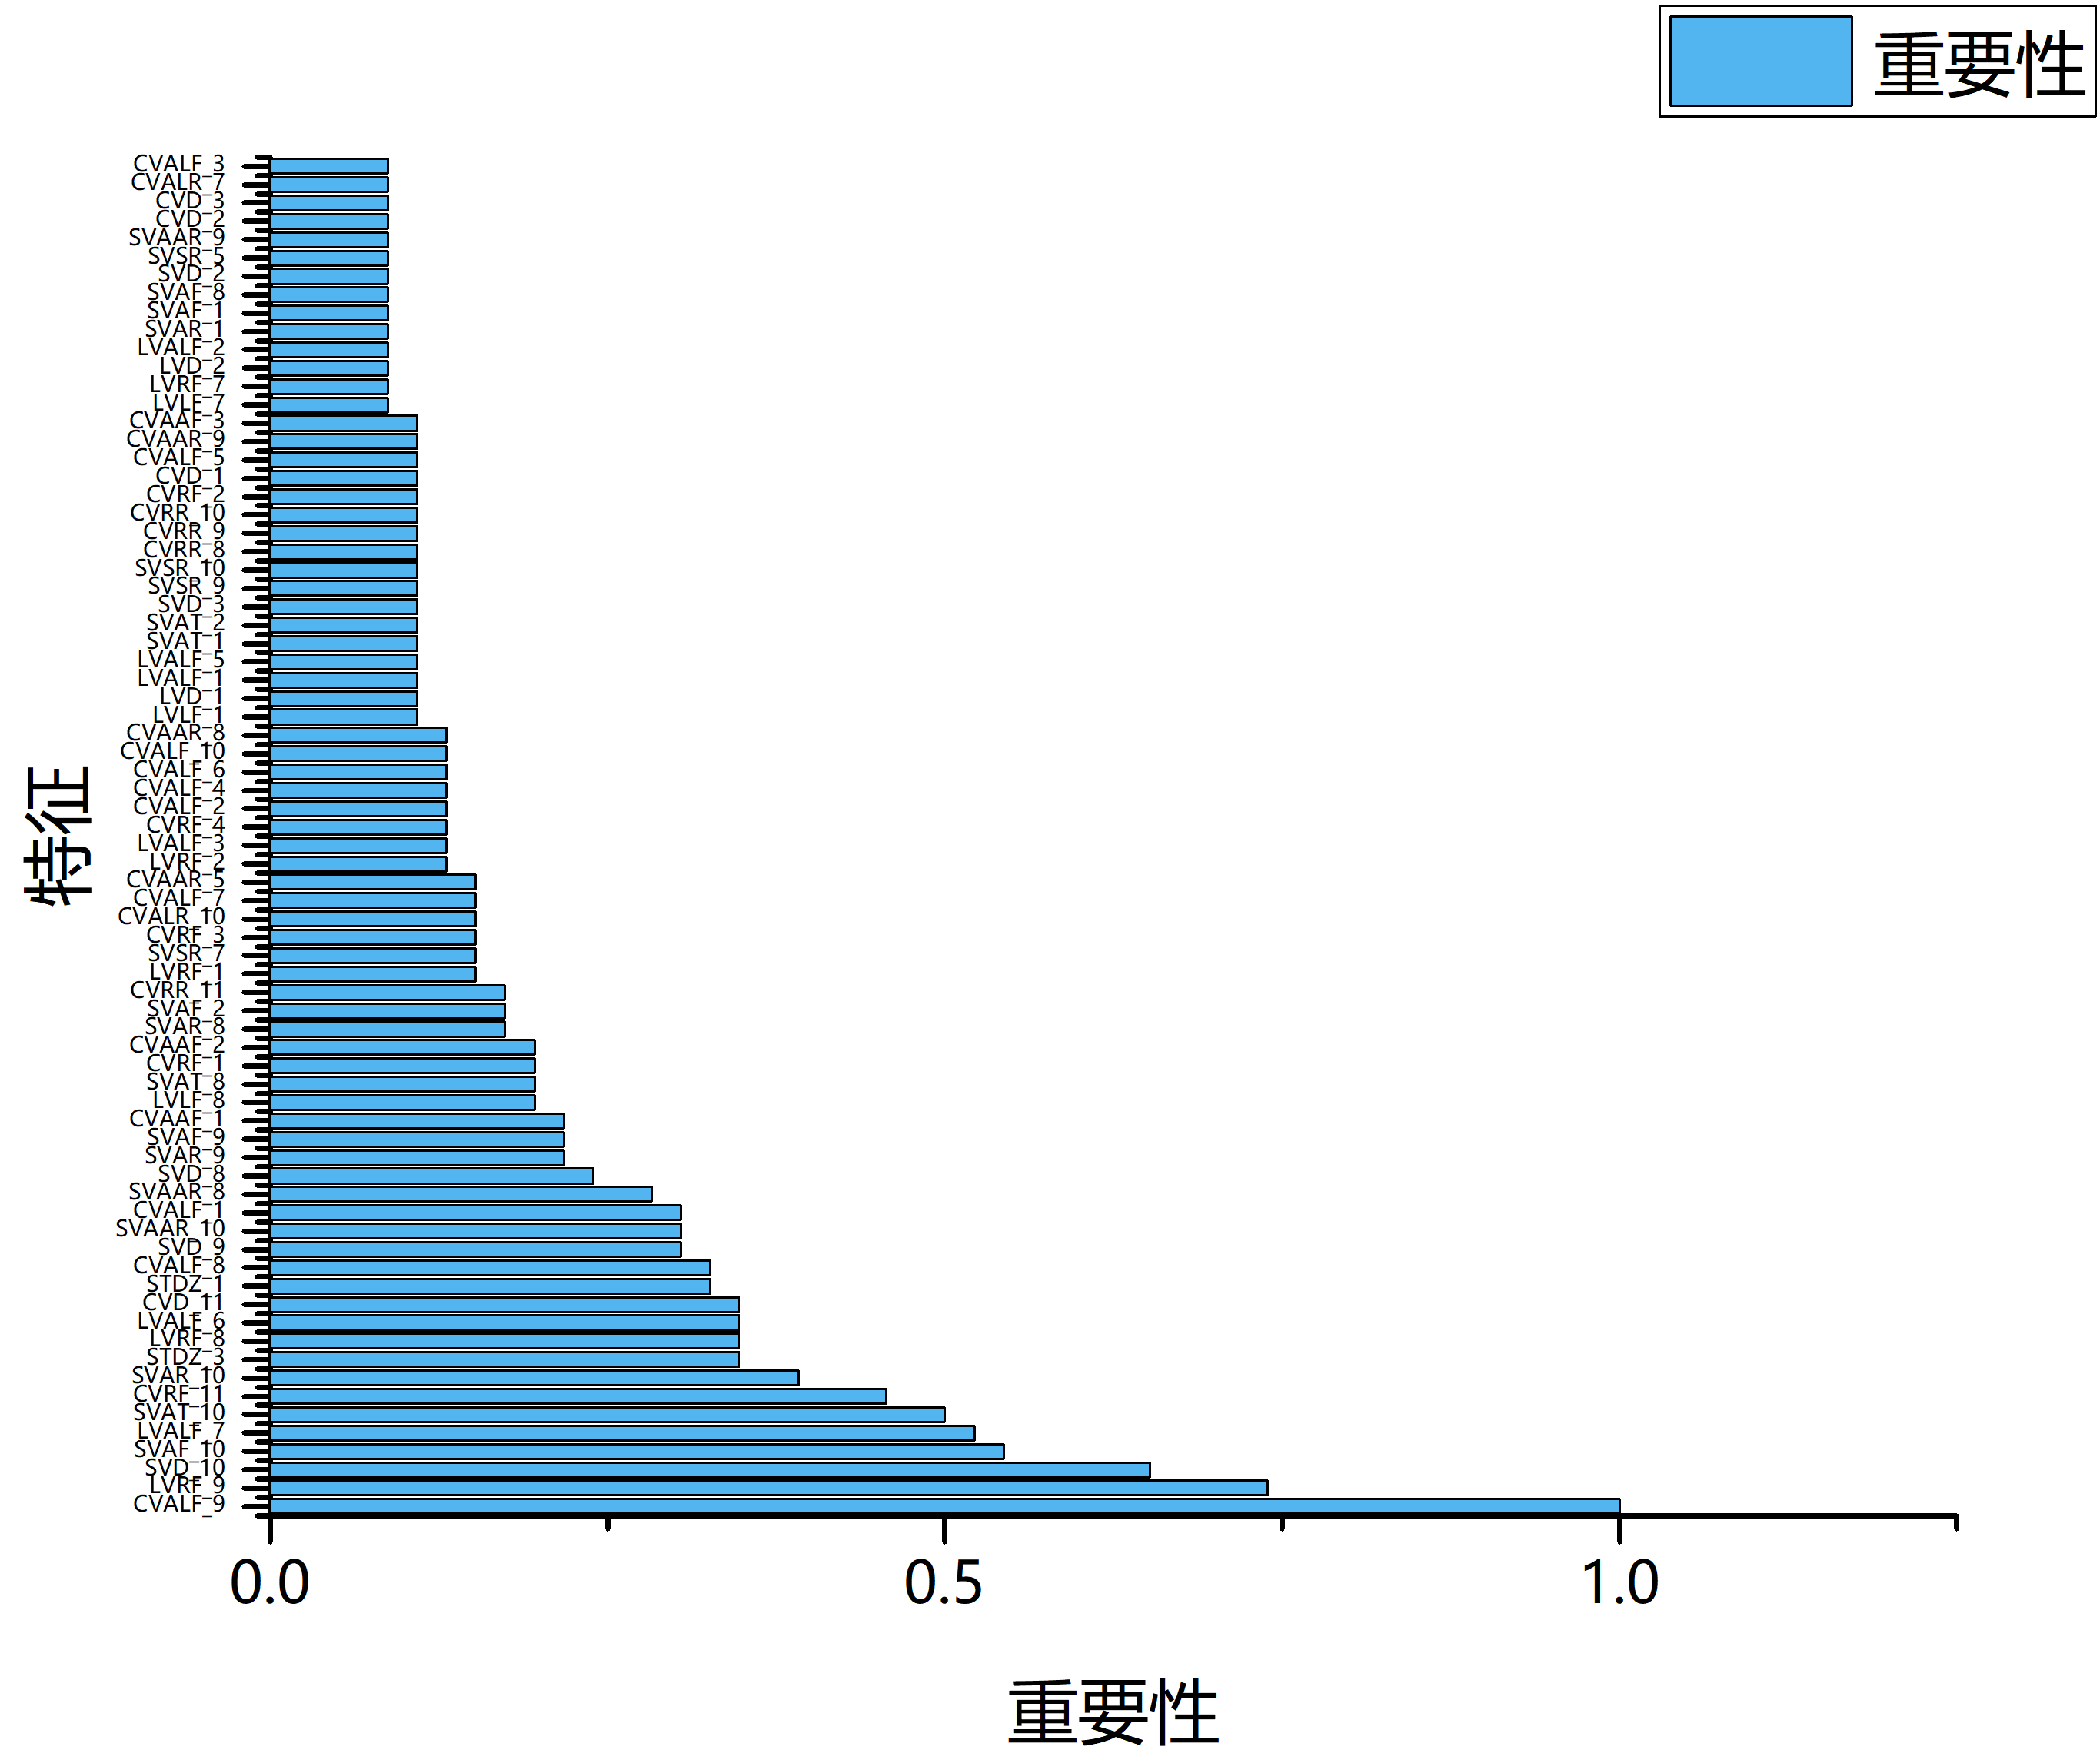
\includegraphics[width=.6\linewidth]{results/rf_ip_pulse_0.7.png}
      \caption[各特征对随机森林的相对贡献度]{\label{fig:rf_importance_pulse}各特征对随机森林的相对贡献度}
\end{figure}

具体特征分析。列举 表格

分析

1 下降支 符合

2 C S 巨多 Ljiaoshao


原始数据特征共有238个,\autoref{fig:rf_importance_pulse}仅保留了
累计贡献度达70\%的74个特征。为进一步考察脉搏波时域特征集\Rnum{1}中特征参数降维的可能性,本研究分别以累计贡献度达全部特征集的70\%的74个特征与50\%的34个特征建立了新的随机森林模型。结果表明,新的随机森林仍然具有非常优秀的性能表现,
在训练集上有着极高的AUC面积值(0.990以上)、测试集上的准确性达97\%。这也说明了本研究进行的降维处理工作是有效的。


\begin{center}
      \zihao{-5}
      \begin{longtable}{m{1.5cm}<{\centering}m{1.5cm}<{\centering}m{1.5cm}<{\centering}m{1.5cm}<{\centering}m{2.5cm}<{\centering}m{1.5cm}<{\centering}m{1.5cm}<{\centering}m{1.5cm}<{\centering}}
            \caption{随机森林对脉搏波特征降维效果}\\
            \label{tab:rf_dr}\\
            \toprule
            % \multicolumn{3}{l}{\multirow{2}{*}{随机森林特征输入}} & \multicolumn{2}{l}{\multirow{2}{*}{训练时间}} & \multicolumn{3}{l}{随机森林性能}        \\
            % \multicolumn{3}{l}{}                          & \multicolumn{2}{l}{}                      & 训练集     & \multicolumn{2}{l}{测试集} \\
            % 特征贡献度比例         & 特征数量        & 特征数量比例        & 训练时间               & 训练时间比例               & AUC     & 混淆矩阵        & 准确率       \\
            \multicolumn{3}{c}{随机森林特征输入} & \multicolumn{2}{c}{训练时间} & 训练集 & \multicolumn{2}{c}{测试集} \\
            特征贡献度比例   & 特征数量   & 特征数量比例  & 训练时间       & 训练时间比例      & AUC & 混淆矩阵        & 准确率       \\
            \midrule
            \endfirsthead
            \caption[]{(续)}\\
            \midrule
            % \\multicolumn{3}{l}{\multirow{2}{*}{随机森林特征输入}} & \multicolumn{2}{l}{\multirow{2}{*}{训练时间}} & \multicolumn{3}{l}{随机森林性能}        \\
            % \multicolumn{3}{l}{}                          & \multicolumn{2}{l}{}                      & 训练集     & \multicolumn{2}{l}{测试集} \\
            % 特征贡献度比例         & 特征数量        & 特征数量比例        & 训练时间               & 训练时间比例               & AUC     & 混淆矩阵        & 准确率       \\
            \multicolumn{3}{c}{随机森林特征输入} & \multicolumn{2}{c}{训练时间} & 训练集 & \multicolumn{2}{c}{测试集} \\
            特征贡献度比例   & 特征数量   & 特征数量比例  & 训练时间       & 训练时间比例      & AUC & 混淆矩阵        & 准确率       \\
            \midrule
            \endhead 
            \midrule
            \endfoot
            \bottomrule
            \endlastfoot
            100.0\%        & 238             &    100.0\%   &     52.06       &     100.0\%     &       0.990               &       $\left[ \begin{array}{cc} 617 & 19 \\ 28 & 909 \end{array} \right]$  &         97.0\%                \\
            70.0\%         & 74              &    31.1\%    &     25.06       &     48.1\%      &    0.993              &     $\left[ \begin{array}{cc} 617 & 19 \\ 26 & 911 \end{array} \right]$        &         97.1\%                \\
            50.0\%         & 34             &   12.0\%      &     16.24       &    31.2\%       &     0.992                  &    $\left[ \begin{array}{cc} 618 & 18 \\ 29 & 908 \end{array} \right]$    &           97.0\%              \\                  
\end{longtable}
\end{center}



4. 分析


基于特征识别判断波形属于正常孕妇或子痫患者
解释

边际效应
过拟合

单个波形影响?

多数波形决定,整体相似度,好像一个意思





二、按照被试人员分层抽样

1. 模型初筛

基于特征识别判断波形属于正常孕妇或子痫患者



数据集划分成了训练集与测试集,其中,训练集上数据按5层交叉验证设计。

2. 参数优化


\begin{landscape}
      \zihao{-5}
      \begin{longtable}{m{3cm}<{\centering}m{1.7cm}<{\centering}m{2.3cm}<{\centering}m{1cm}<{\centering}m{1cm}<{\centering}m{1cm}<{\centering}m{1cm}<{\centering}m{1cm}<{\centering}m{2cm}<{\centering}m{1cm}<{\centering}m{1cm}<{\centering}m{1cm}<{\centering}m{1cm}<{\centering}}
            \caption{初筛结果}\\
            \label{tab:model_screen}\\
            \toprule
            &  & \multicolumn{6}{c}{\textbf{训练集}} & \multicolumn{5}{c}{\textbf{验证集}}                                                                                                                                                                                                      \\
            \multirow{-2}{*}{\textbf{模型类型}} & \multirow{-2}{*}{\textbf{训练时间}} & \textbf{混淆矩阵} &  \textbf{精确率} &  \textbf{召回率} &  \textbf{F1值} &  \textbf{准确率} &  \textbf{AUC} &  \textbf{混淆矩阵} &  \textbf{精确率} &  \textbf{召回率} &  \textbf{F1值} &  \textbf{准确率}    \\
            \midrule
            \endfirsthead
            \caption[]{(续)}\\
            \midrule
            &  & \multicolumn{6}{c}{\textbf{训练集}} & \multicolumn{5}{c}{\textbf{验证集}}                                                                                                                                                                                                      \\
            \multirow{-2}{*}{\textbf{模型类型}} & \multirow{-2}{*}{\textbf{训练时间}} & \textbf{混淆矩阵} &  \textbf{精确率} &  \textbf{召回率} &  \textbf{F1值} &  \textbf{准确率} &  \textbf{AUC} &  \textbf{混淆矩阵} &  \textbf{精确率} &  \textbf{召回率} &  \textbf{F1值} &  \textbf{准确率}    \\
            \midrule
            \endhead 
            \midrule
            \endfoot
            \bottomrule
            \endlastfoot
            K近邻算法      &   4.08 s  &     $\left[ \begin{array}{cc} 2250 & 384 \\ 888 & 2815 \end{array} \right]$ & 88.0\% & 76.0\% &81.6\% & 80.0\% & 0.870 &
            $\left[ \begin{array}{cc} 357 & 190 \\ 141 & 839 \end{array} \right]$ & 81.5\% & 85.6\% & 83.5\% & 78.3\% \\
            决策树算法      &   1.44 s  &     $\left[ \begin{array}{cc} 2062 & 572 \\ 706 & 2997 \end{array} \right]$ & 84.0\% & 80.9\% & 82.4\% & 79.8\% & 0.862 &
            $\left[ \begin{array}{cc} 168 & 379 \\ 136 & 844 \end{array} \right]$ & 69.0\% & 86.1\% & 76.6\% & 66.3\% \\
            随机森林算法      &   50.03 s  &     $\left[ \begin{array}{cc} 2326 & 308 \\ 718 & 2985 \end{array} \right]$ & 90.6\% & 80.6\% & 85.3\% & 83.8\% & 0.929 &
            $\left[ \begin{array}{cc} 317 & 230 \\ 89 & 891 \end{array} \right]$ & 79.5\% & 90.9\% & 84.8\% & 79.1\% \\
            
      \end{longtable}
\end{landscape}

\begin{landscape}
      \zihao{-5}
      \begin{longtable}{m{2cm}<{\centering}m{2cm}<{\centering}m{2cm}<{\centering}m{2cm}<{\centering}m{2cm}<{\centering}m{2cm}<{\centering}m{2cm}<{\centering}m{2cm}<{\centering}m{2cm}<{\centering}}
            \caption{初筛结果}\\
            \label{tab:model_screen}\\
            \toprule
            \multirow{2}{*}{被试孕妇} & \multirow{2}{*}{波形总数} & \multicolumn{2}{c}{K近邻算法} & \multicolumn{2}{c}{决策树} & \multicolumn{2}{c}{随机森林} & \multirow{2}{*}{\begin{tabular}[c]{@{}l@{}}真实子痫前\\ 期患病状态\end{tabular}} \\
                        &                       & 预测阳性数目     & 预测比例       & 预测阳性数目     & 预测比例       & 预测阳性数目     & 预测比例        &                                                                        \\
            \midrule
            \endfirsthead
            \caption[]{(续)}\\
            \midrule
            \multirow{2}{*}{被试孕妇} & \multirow{2}{*}{波形总数} & \multicolumn{2}{c}{K近邻算法} & \multicolumn{2}{c}{决策树} & \multicolumn{2}{c}{随机森林} & \multirow{2}{*}{\begin{tabular}[c]{@{}l@{}}真实子痫前\\ 期患病状态\end{tabular}} \\
                        &                       & 预测阳性数目     & 预测比例       & 预测阳性数目     & 预测比例       & 预测阳性数目     & 预测比例        &                                                                        \\
            \midrule
            \endhead 
            \midrule
            \endfoot
            \bottomrule
            \endlastfoot
            cmf                   & 88                    & 54         & 61.4\%     & 85         & 96.6\%     & 53         & 60.2\%      & 0                                                                      \\
            lxx                   & 63                    & 32         & 50.8\%     & 53         & 84.1\%     & 34         & 54.0\%      & 0                                                                      \\
            shs                   & 112                   & 37         & 33.0\%     & 105        & 93.8\%     & 55         & 49.1\%      & 0                                                                      \\
            sxh                   & 95                    & 27         & 28.4\%     & 64         & 67.4\%     & 21         & 22.1\%      & 0                                                                      \\
            wdq                   & 36                    & 0          & 0.0\%      & 0          & 0.0\%      & 0          & 0.0\%       & 0                                                                      \\
            wsj                   & 78                    & 0          & 0.0\%      & 2          & 2.6\%      & 0          & 0.0\%       & 0                                                                      \\
            ygy                   & 75                    & 40         & 53.3\%     & 70         & 93.3\%     & 67         & 89.3\%      & 0                                                                      \\
            gmn                   & 139                   & 106        & 76.3\%     & 135        & 97.1\%     & 109        & 78.4\%      & 1                                                                      \\
            ty                    & 98                    & 97         & 99.0\%     & 97         & 99.0\%     & 97         & 99.0\%      & 1                                                                      \\
            wjh                   & 86                    & 86         & 100.0\%    & 86         & 100.0\%    & 86         & 100.0\%     & 1                                                                      \\
            xjf                   & 106                   & 23         & 21.7\%     & 59         & 55.7\%     & 87         & 82.1\%      & 1                                                                      \\
            ywy                   & 111                   & 110        & 99.1\%     & 111        & 100.0\%    & 111        & 100.0\%     & 1                                                                      \\
            yxl                   & 110                   & 110        & 100.0\%    & 108        & 98.2\%     & 110        & 100.0\%     & 1                                                                      \\
            zdq                   & 89                    & 81         & 91.0\%     & 84         & 94.4\%     & 82         & 92.1\%      & 1                                                                      \\
            zl                    & 152                   & 137        & 90.1\%     & 75         & 49.3\%     & 120        & 78.9\%      & 1                                                                      \\
            zyy                   & 89                    & 89         & 100.0\%    & 89         & 100.0\%    & 89         & 100.0\%     & 1                                                                       \\    
\end{longtable}
\end{landscape}

超参数调优

4. 分析




\subsection{基于脉搏波时域特征集\Rnum{2}的结果及分析}

一、按照全波波形抽样

\begin{landscape}
      \zihao{-5}
      \begin{longtable}{m{3cm}<{\centering}m{1.7cm}<{\centering}m{2.3cm}<{\centering}m{1cm}<{\centering}m{1cm}<{\centering}m{1cm}<{\centering}m{1cm}<{\centering}m{1cm}<{\centering}m{2cm}<{\centering}m{1cm}<{\centering}m{1cm}<{\centering}m{1cm}<{\centering}m{1cm}<{\centering}}
            \caption{初筛结果}\\
            \label{tab:model_screen}\\
            \toprule
            &  & \multicolumn{6}{c}{\textbf{训练集}} & \multicolumn{5}{c}{\textbf{验证集}}                                                                                                                                                                                                      \\
            \multirow{-2}{*}{\textbf{模型类型}} & \multirow{-2}{*}{\textbf{训练时间}} & \textbf{混淆矩阵} &  \textbf{精确率} &  \textbf{召回率} &  \textbf{F1值} &  \textbf{准确率} &  \textbf{AUC} &  \textbf{混淆矩阵} &  \textbf{精确率} &  \textbf{召回率} &  \textbf{F1值} &  \textbf{准确率}    \\
            \midrule
            \endfirsthead
            \caption[]{(续)}\\
            \midrule
            &  & \multicolumn{6}{c}{\textbf{训练集}} & \multicolumn{5}{c}{\textbf{验证集}}                                                                                                                                                                                                      \\
            \multirow{-2}{*}{\textbf{模型类型}} & \multirow{-2}{*}{\textbf{训练时间}} & \textbf{混淆矩阵} &  \textbf{精确率} &  \textbf{召回率} &  \textbf{F1值} &  \textbf{准确率} &  \textbf{AUC} &  \textbf{混淆矩阵} &  \textbf{精确率} &  \textbf{召回率} &  \textbf{F1值} &  \textbf{准确率}    \\
            \midrule
            \endhead 
            \midrule
            \endfoot
            \bottomrule
            \endlastfoot
            决策树算法      &   1.31 s  &     $\left[ \begin{array}{cc} 1220 & 1325 \\ 604 & 3142 \end{array} \right]$ & 70.3\% & 83.9\% &76.5\% & 69.3\% & 0.743 &
            $\left[ \begin{array}{cc} 227 & 409 \\ 78 & 859 \end{array} \right]$ & 67.8\% & 91.7\% & 77.9\% & 69.0\% \\
            K近邻算法      &   2.93 s  &     $\left[ \begin{array}{cc} 1515 & 1030 \\ 607 & 3139 \end{array} \right]$ & 75.2\% & 83.8\% & 79.3\% & 74.03\% & 0.810 &
            $\left[ \begin{array}{cc} 381 & 255 \\ 142 & 799 \end{array} \right]$ & 75.7\% & 84.8\% & 80.0\% & 74.8\% \\
            随机森林算法      &   1.45 s  &     $\left[ \begin{array}{cc} 1220 & 1325 \\ 604 & 3142 \end{array} \right]$ & 70.3\% & 83.9\% & 76.5\% & 69.3\% & 0.743 &
            $\left[ \begin{array}{cc} 227 & 409 \\ 78 & 859 \end{array} \right]$ & 67.7\% & 91.7\% & 77.9\% & 69.0\% \\
            
      \end{longtable}
\end{landscape}





\section{非监督学习算法的具体表现及分析}
聚类分析是无监督学习的一种,旨在发现数据间是否有潜在的相似性\cite{Liu2018,Li2017}。
因此,我们做了额外的探究——在不给定脉搏波对应的子痫前期的数据标签的基础上,探究能否有效的将数据分成两类,并考察验证分类的效果。

本文进行了以下探究:
1.	分别使用基于ppg 特征的$ppg_feature$ 数据与基于ppg波形数据的$ppg_points $数据,使用sklearn的kmeans 方法进行了聚类分析,其中超参数$n_clusters$被设置为2。
此时,此时若我们将聚类结果作为其学习的分类结果,与数据对应的数据标签进行对照,也可以得到混淆矩阵分别如下

之所以每种分析会得到两个混淆矩阵,是因为聚类分析的簇是不带标签的。两个混淆矩阵是给予簇不同的标签(健康或子痫)。为分析方便,我们选取准确率高的一种聚类结果,即上表中的2、3。并在此基础上进行后续分析。

2.	从表格中可以看到两种数据的聚类分析的准确率分别达到了61.6\%与51.5\%。
基于特征的聚类效果优于直接使用脉搏波波形数据的。
其次,乍一看,数据分类效果并不太好。特别是后者的准确率堪堪超过50\%(典型的随机分类的效果)
但是,我们需要注意到聚类分析的本质是根据数据特征的相似度,也即数据波形的相似度。
因此,让我们来考察下划分出来的波形究竟如何。
于是,我们把图画出来。

此外,我们还需要注意到另外一个变量因素,在PE的影响下,所有患病孕妇的数据波形是会受到影响的,而与正常波形形态有异。因此,所有PE患者都受到了一定程序的医学干预(包括不限于降血压等治疗),目的是使PE患者能够恢复正常水平。因此,会出现假阴性远高于假阳性的现象。可以总结为,在PE确实能改变孕妇脉搏波波形的前提下,聚类分析中出现的假阴性高于假阳性证明是医学干预的必然结果。分析数据与理论分析保持一致。
3.	到具体波形

\begin{figure}[htbp]
    \centering
    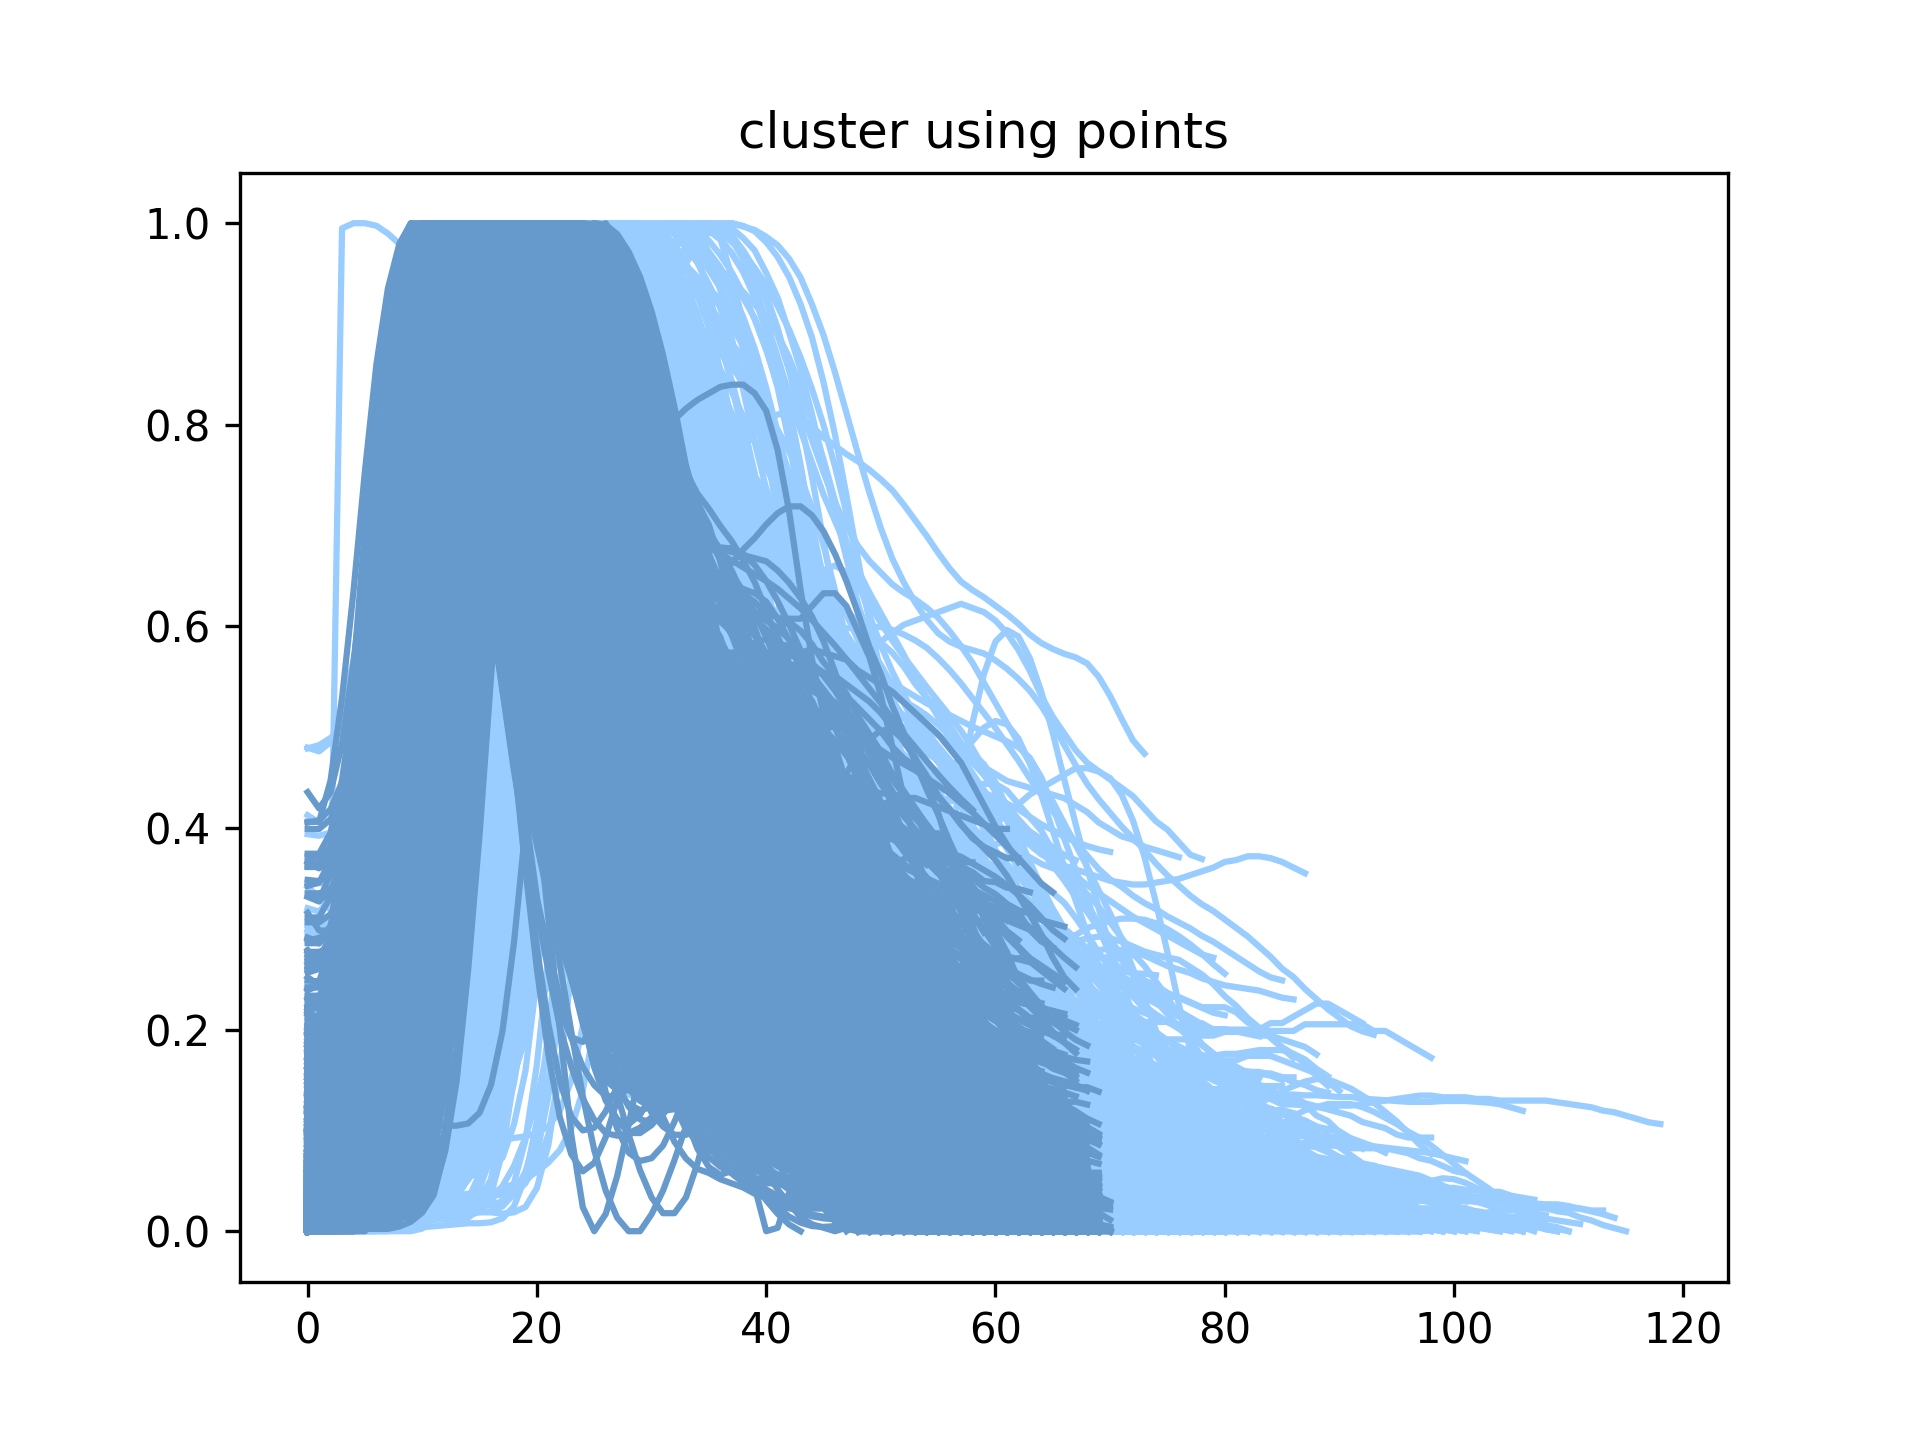
\includegraphics[width=.6\linewidth]{unsupervised/cluster using points_2d}
    \caption[]{\label{fig:cluster2d}111}
\end{figure}
\begin{figure}[htbp]
    \centering
    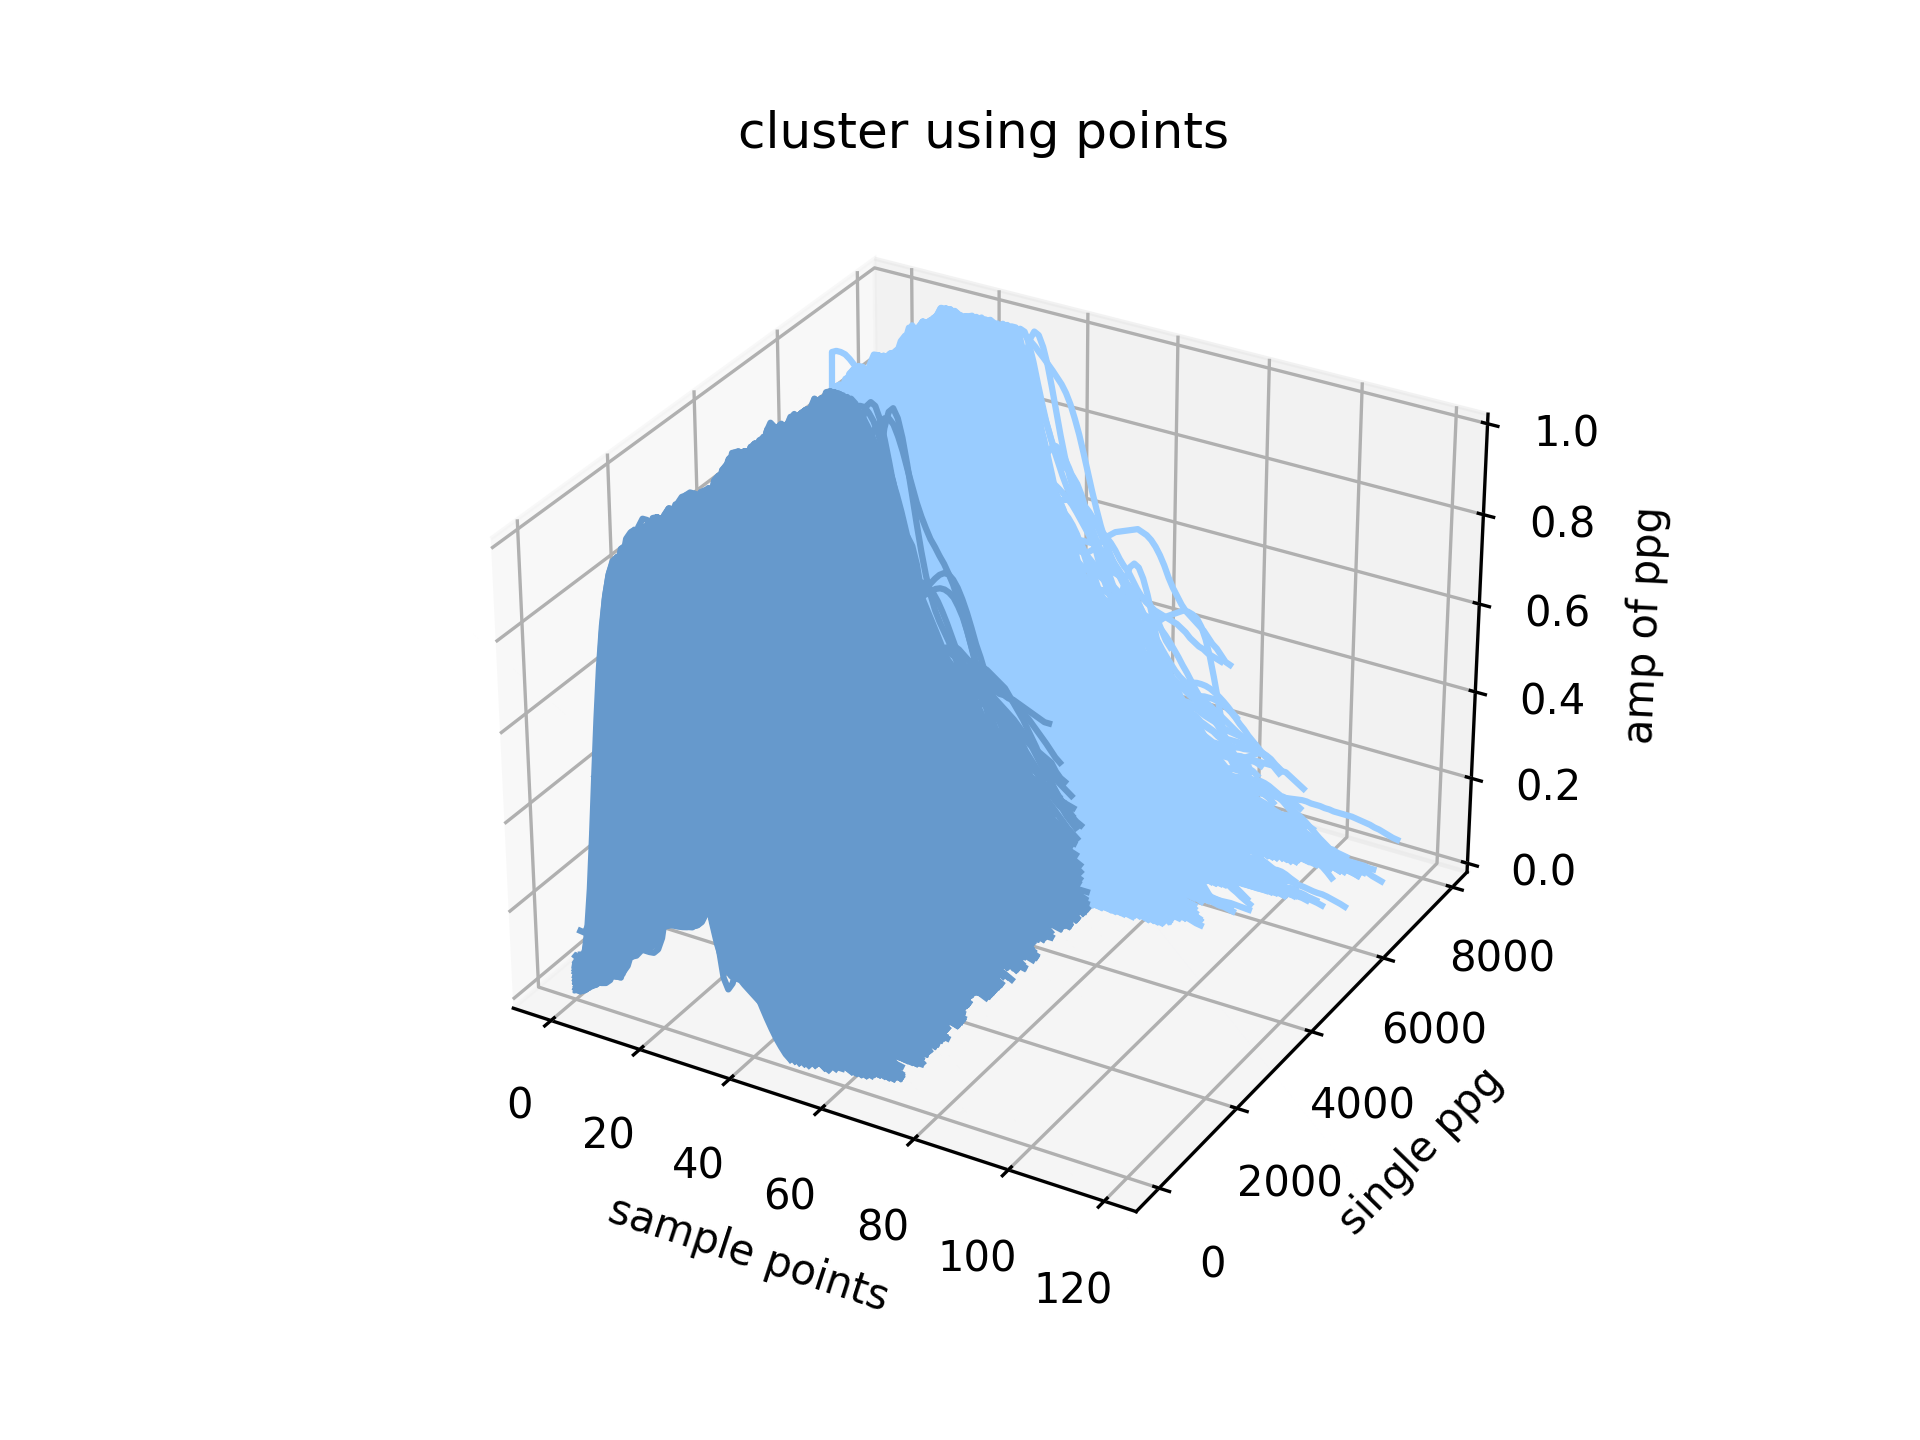
\includegraphics[width=.7\linewidth]{unsupervised/cluster using points_3d}
    \caption[]{\label{fig:cluster3d}222}
\end{figure}
\section{对k的调整与探索}
\section{分析与结论}
\section{小结}